% Options for packages loaded elsewhere
\PassOptionsToPackage{unicode}{hyperref}
\PassOptionsToPackage{hyphens}{url}
%
\documentclass[
]{book}
\usepackage{lmodern}
\usepackage{amsmath}
\usepackage{ifxetex,ifluatex}
\ifnum 0\ifxetex 1\fi\ifluatex 1\fi=0 % if pdftex
  \usepackage[T1]{fontenc}
  \usepackage[utf8]{inputenc}
  \usepackage{textcomp} % provide euro and other symbols
  \usepackage{amssymb}
\else % if luatex or xetex
  \usepackage{unicode-math}
  \defaultfontfeatures{Scale=MatchLowercase}
  \defaultfontfeatures[\rmfamily]{Ligatures=TeX,Scale=1}
\fi
% Use upquote if available, for straight quotes in verbatim environments
\IfFileExists{upquote.sty}{\usepackage{upquote}}{}
\IfFileExists{microtype.sty}{% use microtype if available
  \usepackage[]{microtype}
  \UseMicrotypeSet[protrusion]{basicmath} % disable protrusion for tt fonts
}{}
\makeatletter
\@ifundefined{KOMAClassName}{% if non-KOMA class
  \IfFileExists{parskip.sty}{%
    \usepackage{parskip}
  }{% else
    \setlength{\parindent}{0pt}
    \setlength{\parskip}{6pt plus 2pt minus 1pt}}
}{% if KOMA class
  \KOMAoptions{parskip=half}}
\makeatother
\usepackage{xcolor}
\IfFileExists{xurl.sty}{\usepackage{xurl}}{} % add URL line breaks if available
\IfFileExists{bookmark.sty}{\usepackage{bookmark}}{\usepackage{hyperref}}
\hypersetup{
  pdftitle={TIES Measurement Report Automation Project},
  pdfauthor={Michael Wu},
  hidelinks,
  pdfcreator={LaTeX via pandoc}}
\urlstyle{same} % disable monospaced font for URLs
\usepackage{longtable,booktabs}
\usepackage{calc} % for calculating minipage widths
% Correct order of tables after \paragraph or \subparagraph
\usepackage{etoolbox}
\makeatletter
\patchcmd\longtable{\par}{\if@noskipsec\mbox{}\fi\par}{}{}
\makeatother
% Allow footnotes in longtable head/foot
\IfFileExists{footnotehyper.sty}{\usepackage{footnotehyper}}{\usepackage{footnote}}
\makesavenoteenv{longtable}
\usepackage{graphicx}
\makeatletter
\def\maxwidth{\ifdim\Gin@nat@width>\linewidth\linewidth\else\Gin@nat@width\fi}
\def\maxheight{\ifdim\Gin@nat@height>\textheight\textheight\else\Gin@nat@height\fi}
\makeatother
% Scale images if necessary, so that they will not overflow the page
% margins by default, and it is still possible to overwrite the defaults
% using explicit options in \includegraphics[width, height, ...]{}
\setkeys{Gin}{width=\maxwidth,height=\maxheight,keepaspectratio}
% Set default figure placement to htbp
\makeatletter
\def\fps@figure{htbp}
\makeatother
\setlength{\emergencystretch}{3em} % prevent overfull lines
\providecommand{\tightlist}{%
  \setlength{\itemsep}{0pt}\setlength{\parskip}{0pt}}
\setcounter{secnumdepth}{5}
\usepackage{booktabs}
\usepackage{amsthm}
\makeatletter
\def\thm@space@setup{%
  \thm@preskip=8pt plus 2pt minus 4pt
  \thm@postskip=\thm@preskip
}
\makeatother
\ifluatex
  \usepackage{selnolig}  % disable illegal ligatures
\fi
\usepackage[]{natbib}
\bibliographystyle{apalike}

\title{TIES Measurement Report Automation Project}
\author{Michael Wu}
\date{2021-03-29}

\begin{document}
\maketitle

{
\setcounter{tocdepth}{1}
\tableofcontents
}
\hypertarget{project-overview}{%
\chapter{Project overview}\label{project-overview}}

This project is developed to generate lengthy but informative measurement reports from survey data and Mplus measurement model outputs for projects at \href{https://steinhardt.nyu.edu/ihdsc/global-ties}{NYU Global TIES for Children}.

Typically, a research institute like TIES has the obligation to generate detailed measurement reports to better inform the funders and the cooperating agencies about its most up-to-date work. However, even with a Word template, the process from analytical results to a publishable report is \underline{\textbf{unnecessarily inefficent and prone to mistakes}} even for the most careful research assistant.

Therefore, we develop an R package called \href{https://github.com/nyuglobalties/mrautomatr}{\texttt{mrautomatr}} to be used in conjunction with Rstudio to address this issue. Currently, the project only suits the need of NYU Global TIES, where we can impose \href{https://nyu.box.com/s/ate5l7wmw164u7xjg3g8x1vrfhwnt0ax}{naming rules} for files and variables and most people use Mplus for measurement modeling and STATA for other analyses. Future adaptations are needed as people move their analysis to R.

The project workflow is shown below: the users specify parameters in a Microsoft excel sheet and move several files to a destined folder, run a command in R, and (\textbf{boom!}) there is a well-formatted measurement report in Microsoft Word (powered by the \href{https://davidgohel.github.io/flextable/}{\texttt{flextable}} \& \href{https://bookdown.org/yihui/rmarkdown/}{\texttt{rmarkdown}} R packages).

\begin{center}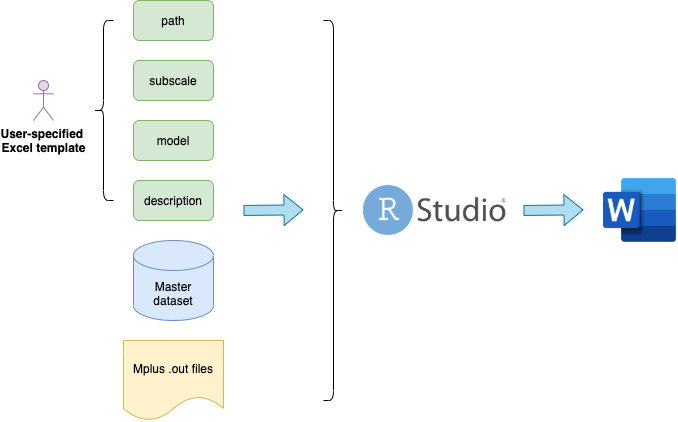
\includegraphics[width=0.66\linewidth]{images/mrautomatr_diagram} \end{center}

We chose Word over LaTex (which generates pdf files) and html (which generates web pages) simply to minimize the confusion around writing codes in R, which takes a long time to learn. After generating the reproducible parts of the report, feel free to rename it and manually edit the sections that are text-heavy.

Check out the \href{https://github.com/nyuglobalties/workshops}{TIES R workshop series} and Yihui Xie's \href{https://bookdown.org/yihui/rmarkdown/}{Rmarkdown book} if you'd like to learn some necessary tools to customize your reporting formats using R.

\hypertarget{set-up-the-package}{%
\chapter{Set up the package}\label{set-up-the-package}}

\hypertarget{install-the-necessary-softwares}{%
\section{Install the necessary softwares}\label{install-the-necessary-softwares}}

You need to set up \texttt{R} and \texttt{Rstudio} on your computer before everything. \texttt{R} is the programming language that powers this project, and \texttt{Rstudio} is the interface that allows you better interact with your R code. Please follow the steps below:

\begin{itemize}
\tightlist
\item
  Download \texttt{R} \href{https://cran.r-project.org/mirrors.html}{here} and install it before you install \texttt{Rstudio}.
\item
  Download \texttt{Rstudio} \href{https://rstudio.com/products/rstudio/download/\#download}{here} and install it.
\item
  Open Rstudio, and click the first icon from the left on the Rstudio toolbar, and select R Markdown. Rstudio will prompt you to install several packages, just follow the instructions and install them.
\end{itemize}

\hypertarget{download-and-install-the-mrautomatr-package}{%
\section{\texorpdfstring{Download and install the \texttt{mrautomatr} package}{Download and install the mrautomatr package}}\label{download-and-install-the-mrautomatr-package}}

\begin{itemize}
\tightlist
\item
  Run the following lines:
\end{itemize}

\begin{verbatim}
install.packages("usethis")
install.packages("devtools")
library(usethis)
library(devtools)
\end{verbatim}

\begin{itemize}
\item
  Set up your GitHub Personal Auth Token set following instructions on \href{https://usethis.r-lib.org/reference/browse_github_pat.html}{this website}. This is only applicable to this package right now since it's internal and private. You may need to email Patrick Anker in order to gain access to the TIES github repository.
\item
  Run the following line:
\end{itemize}

\begin{verbatim}
devtools::install_github("nyuglobalties/mrautomatr")
library(mrautomatr)
\end{verbatim}

\begin{itemize}
\tightlist
\item
  Check out the functions by running \texttt{?function\_name}, e.g.:
\end{itemize}

\begin{verbatim}
?mrautomatr
\end{verbatim}

\hypertarget{set-up-the-parameters}{%
\chapter{Set up the parameters}\label{set-up-the-parameters}}

\hypertarget{organize-your-model-outputs}{%
\section{Organize your model outputs}\label{organize-your-model-outputs}}

Before you run any R codes, you need to make sure that the parameters for the report are correctly specified.

First, copy and paste all \textbf{currently available} final Mplus models (only the \texttt{.out} files) into one folder (e.g.~a folder called \texttt{Measurement\ report/Models} somewhere on Box). This includes:

\begin{itemize}
\tightlist
\item
  EFA models
\item
  CFA models
\item
  Longitudinal invariance models
\item
  Treatment invariance models
\item
  Age invariance models
\item
  Gender invariance models
\end{itemize}

\hypertarget{fill-in-the-excel-template}{%
\section{Fill in the excel template}\label{fill-in-the-excel-template}}

Second, fill in the excel sheet template that we provide. This excel file is downloaded along with the \texttt{mrautomatr} package. You can find its file path on your computer by running \texttt{system.file("templates",\ "input\_template.xlsx",\ package\ =\ "mrautomatr")} in R. Copy and paste it somewhere in your computer (e.g.~a folder called \texttt{Measurement\ report/template}).

Alternatively, you can also find this template (\texttt{input\_template.xlsx}) located in \texttt{inst/templates/} in the \href{https://github.com/nyuglobalties/mrautomatr}{package GitHub repository}. Simply hit \texttt{Download} to download the template and store somewhere in your computer.

In this template, you need to manually type in the following parameters. For any parameters that are not available temporarily, you can leave blank and still be able to generate the report (with errors in the Word document telling you that you need to specify more parameters to have a full report).

\hypertarget{tab-1-path}{%
\subsection{\texorpdfstring{Tab 1: \texttt{path}}{Tab 1: path}}\label{tab-1-path}}

A shorthand to get file path on Mac: go to the path/file and hit \texttt{command\ +\ option\ +\ C}.

\begin{itemize}
\item
  \texttt{year} will show up in the first line of your document (not the title).
\item
  \texttt{measure} will show up in the first line of your document.
\item
  \texttt{data\_file\_path} should be wherever the final master data is located. It will be used to calculate summary statistics and bivariate correlations. Our tool currently takes the following data formats: \texttt{.csv}, \texttt{.xlsx}, \texttt{.dta}.
\item
  \texttt{fs\_data\_file\_path} refers to the file path where the tabular data of the Mplus-generated factor scores is saved. Because Mplus \textbf{does not} generate a spreadsheet, you will need to:

  \begin{itemize}
  \item
    \textbf{(1) copy and paste the factor scores into an excel sheet, and}
  \item
    \textbf{(2) insert the first row and name the variables exactly the same as they are in your master dataset and in your other Mplus models.}
  \item
    \textbf{(3) save the sheet either as a .csv or an .xlsx file.}
  \end{itemize}
\item
  \texttt{model\_file\_path} leads you to all the Mplus outputs.
\end{itemize}

\hypertarget{tab-2-subscale}{%
\subsection{\texorpdfstring{Tab 2: \texttt{subscale}}{Tab 2: subscale}}\label{tab-2-subscale}}

\begin{itemize}
\item
  The first row should contain the subscale/factor names. They should be the same as the ones in your Mplus models.
\item
  For each subscale/factor, list the items. The rows can be of unequal length (i.e.~you can leave blanks for subscales with smaller number of items).
\item
  These are specified to generate reliability estimates from the master dataset.
\end{itemize}

\hypertarget{tab-3-model}{%
\subsection{\texorpdfstring{Tab 3: \texttt{model}}{Tab 3: model}}\label{tab-3-model}}

\begin{itemize}
\item
  This specifies all necessary Mplus model names (i.e.~\texttt{xxx.out}).
\item
  List all available models in the order of waves (e.g.~wave 1 before wave 2).
\item
  There is no restrictions on the file names, but please follow the \href{https://nyu.box.com/s/ate5l7wmw164u7xjg3g8x1vrfhwnt0ax}{naming rules} for reproducibility purposes.
\end{itemize}

\hypertarget{tab-4-description}{%
\subsection{\texorpdfstring{Tab 4: \texttt{description}}{Tab 4: description}}\label{tab-4-description}}

\begin{itemize}
\item
  This is specified to have a description of the items at the beginning of the report.
\item
  You can format this tab in any ways that you like, but the caveat is that (1) the first row will be taken as the header and set to bold, and (2) you cannot merge cells.
\end{itemize}

\begin{longtable}[]{@{}ll@{}}
\toprule
\begin{minipage}[b]{(\columnwidth - 1\tabcolsep) * \real{0.25}}\raggedright
Variable name\strut
\end{minipage} & \begin{minipage}[b]{(\columnwidth - 1\tabcolsep) * \real{0.75}}\raggedright
Description\strut
\end{minipage}\tabularnewline
\midrule
\endhead
\begin{minipage}[t]{(\columnwidth - 1\tabcolsep) * \real{0.25}}\raggedright
\texttt{year}\strut
\end{minipage} & \begin{minipage}[t]{(\columnwidth - 1\tabcolsep) * \real{0.75}}\raggedright
Study site and year\strut
\end{minipage}\tabularnewline
\begin{minipage}[t]{(\columnwidth - 1\tabcolsep) * \real{0.25}}\raggedright
\texttt{measure}\strut
\end{minipage} & \begin{minipage}[t]{(\columnwidth - 1\tabcolsep) * \real{0.75}}\raggedright
Measure name\strut
\end{minipage}\tabularnewline
\begin{minipage}[t]{(\columnwidth - 1\tabcolsep) * \real{0.25}}\raggedright
\texttt{data\_file\_path}\strut
\end{minipage} & \begin{minipage}[t]{(\columnwidth - 1\tabcolsep) * \real{0.75}}\raggedright
Local file path to the master dataset on your own computer\strut
\end{minipage}\tabularnewline
\begin{minipage}[t]{(\columnwidth - 1\tabcolsep) * \real{0.25}}\raggedright
\texttt{fs\_data\_file\_path}\strut
\end{minipage} & \begin{minipage}[t]{(\columnwidth - 1\tabcolsep) * \real{0.75}}\raggedright
Local file path to the factor score dataset on your own computer\strut
\end{minipage}\tabularnewline
\begin{minipage}[t]{(\columnwidth - 1\tabcolsep) * \real{0.25}}\raggedright
\texttt{model\_file\_path}\strut
\end{minipage} & \begin{minipage}[t]{(\columnwidth - 1\tabcolsep) * \real{0.75}}\raggedright
Local file path to all the Mplus .out files\strut
\end{minipage}\tabularnewline
\begin{minipage}[t]{(\columnwidth - 1\tabcolsep) * \real{0.25}}\raggedright
\texttt{subscale}\strut
\end{minipage} & \begin{minipage}[t]{(\columnwidth - 1\tabcolsep) * \real{0.75}}\raggedright
Subscales and their corresponding items\strut
\end{minipage}\tabularnewline
\begin{minipage}[t]{(\columnwidth - 1\tabcolsep) * \real{0.25}}\raggedright
\texttt{model\_efa}\strut
\end{minipage} & \begin{minipage}[t]{(\columnwidth - 1\tabcolsep) * \real{0.75}}\raggedright
EFA models\strut
\end{minipage}\tabularnewline
\begin{minipage}[t]{(\columnwidth - 1\tabcolsep) * \real{0.25}}\raggedright
\texttt{model\_cfa}\strut
\end{minipage} & \begin{minipage}[t]{(\columnwidth - 1\tabcolsep) * \real{0.75}}\raggedright
CFA models\strut
\end{minipage}\tabularnewline
\begin{minipage}[t]{(\columnwidth - 1\tabcolsep) * \real{0.25}}\raggedright
\texttt{model\_inv\_tx}\strut
\end{minipage} & \begin{minipage}[t]{(\columnwidth - 1\tabcolsep) * \real{0.75}}\raggedright
Treatment invariance models\strut
\end{minipage}\tabularnewline
\begin{minipage}[t]{(\columnwidth - 1\tabcolsep) * \real{0.25}}\raggedright
\texttt{model\_inv\_gender}\strut
\end{minipage} & \begin{minipage}[t]{(\columnwidth - 1\tabcolsep) * \real{0.75}}\raggedright
Gender invariance models\strut
\end{minipage}\tabularnewline
\begin{minipage}[t]{(\columnwidth - 1\tabcolsep) * \real{0.25}}\raggedright
\texttt{model\_inv\_age}\strut
\end{minipage} & \begin{minipage}[t]{(\columnwidth - 1\tabcolsep) * \real{0.75}}\raggedright
Age invariance models\strut
\end{minipage}\tabularnewline
\begin{minipage}[t]{(\columnwidth - 1\tabcolsep) * \real{0.25}}\raggedright
\texttt{model\_inv\_lg}\strut
\end{minipage} & \begin{minipage}[t]{(\columnwidth - 1\tabcolsep) * \real{0.75}}\raggedright
Longitudinal invariance model\strut
\end{minipage}\tabularnewline
\begin{minipage}[t]{(\columnwidth - 1\tabcolsep) * \real{0.25}}\raggedright
\texttt{description}\strut
\end{minipage} & \begin{minipage}[t]{(\columnwidth - 1\tabcolsep) * \real{0.75}}\raggedright
Detailed item descriptions\strut
\end{minipage}\tabularnewline
\bottomrule
\end{longtable}

\hypertarget{generate-the-report}{%
\chapter{Generate the report}\label{generate-the-report}}

After carefully setting your parameters, you can now generate your report!

There are three ways to generate reports:

\begin{enumerate}
\def\labelenumi{\arabic{enumi}.}
\item
  Generate one report for one measure using the default settings \texttt{render\_report()}
\item
  Generate one report for one measure using customized settings by the users \texttt{render\_report\_manual()}
\item
  Generate multiple separate reports for multiple measures using default settings \texttt{render\_report\_multiple()}
\end{enumerate}

After generating the report, make sure to rename it and manually edit the sections that are text-heavy. The renaming is necessary because you may accidentally overwrite your manual edits if you regenerate the report in R.

Rmarkdown is not powerful yet to allow back-translation from Word to R codes, so your manual changes in Word will not be reflected in the R codes when you regenerate the report for some reasons (e.g.~wrong file names). So we recommend finalizing the tables and plots before you write texts in the Word document (or you can just store the texts in another and move them over to the master report whenever you feel ready).

\hypertarget{render_report}{%
\section{\texorpdfstring{\texttt{render\_report()}}{render\_report()}}\label{render_report}}

Run \texttt{?render\_report()} to see what each argument represents.

Example:

\begin{verbatim}
render_report(input_dir = "/Users/michaelfive/Google Drive/NYU/3EA/test",
              template = "input_template_lebanon_cs.xlsx",
              index = "lebanon_cs",
              title = "Lebanon Year 1 (2016-2017)",
              output_dir = "/Users/michaelfive/Google Drive/NYU/3EA/test")
\end{verbatim}

This function renders one report for the specified measure.

\hypertarget{render_report_manual}{%
\section{\texorpdfstring{\texttt{render\_report\_manual()}}{render\_report\_manual()}}\label{render_report_manual}}

Run \texttt{?render\_report\_manual()} to see what each argument represents.

Example:

\begin{verbatim}
render_report_manual(index = "lebanon_cs",
                     output_dir = "/Users/michaelfive/Google Drive/NYU/3EA/test")
\end{verbatim}

This function opens a Shiny web page where you can click/unclick sections you'd like to include/exclude in the report (see descriptions below). It also renders one report for the specified measure.

\begin{longtable}[]{@{}ll@{}}
\toprule
\begin{minipage}[b]{(\columnwidth - 1\tabcolsep) * \real{0.13}}\raggedright
Parameters\strut
\end{minipage} & \begin{minipage}[b]{(\columnwidth - 1\tabcolsep) * \real{0.87}}\raggedright
Description\strut
\end{minipage}\tabularnewline
\midrule
\endhead
\begin{minipage}[t]{(\columnwidth - 1\tabcolsep) * \real{0.13}}\raggedright
\texttt{printcode}\strut
\end{minipage} & \begin{minipage}[t]{(\columnwidth - 1\tabcolsep) * \real{0.87}}\raggedright
whether you'd like R codes to be printed in your document\strut
\end{minipage}\tabularnewline
\begin{minipage}[t]{(\columnwidth - 1\tabcolsep) * \real{0.13}}\raggedright
\texttt{printwarning}\strut
\end{minipage} & \begin{minipage}[t]{(\columnwidth - 1\tabcolsep) * \real{0.87}}\raggedright
whether you'd like to print warnings in running the codes\strut
\end{minipage}\tabularnewline
\begin{minipage}[t]{(\columnwidth - 1\tabcolsep) * \real{0.13}}\raggedright
\texttt{storecache}\strut
\end{minipage} & \begin{minipage}[t]{(\columnwidth - 1\tabcolsep) * \real{0.87}}\raggedright
whether you'd like to store \texttt{knitr} cache (only for programming purposes, see \href{https://bookdown.org/yihui/rmarkdown-cookbook/cache.html}{here})\strut
\end{minipage}\tabularnewline
\begin{minipage}[t]{(\columnwidth - 1\tabcolsep) * \real{0.13}}\raggedright
\texttt{set\_title}\strut
\end{minipage} & \begin{minipage}[t]{(\columnwidth - 1\tabcolsep) * \real{0.87}}\raggedright
title\strut
\end{minipage}\tabularnewline
\begin{minipage}[t]{(\columnwidth - 1\tabcolsep) * \real{0.13}}\raggedright
\texttt{set\_author}\strut
\end{minipage} & \begin{minipage}[t]{(\columnwidth - 1\tabcolsep) * \real{0.87}}\raggedright
author\strut
\end{minipage}\tabularnewline
\begin{minipage}[t]{(\columnwidth - 1\tabcolsep) * \real{0.13}}\raggedright
\texttt{template}\strut
\end{minipage} & \begin{minipage}[t]{(\columnwidth - 1\tabcolsep) * \real{0.87}}\raggedright
parameter template file path\strut
\end{minipage}\tabularnewline
\begin{minipage}[t]{(\columnwidth - 1\tabcolsep) * \real{0.13}}\raggedright
\texttt{item}\strut
\end{minipage} & \begin{minipage}[t]{(\columnwidth - 1\tabcolsep) * \real{0.87}}\raggedright
print item descriptions\strut
\end{minipage}\tabularnewline
\begin{minipage}[t]{(\columnwidth - 1\tabcolsep) * \real{0.13}}\raggedright
\texttt{descriptive}\strut
\end{minipage} & \begin{minipage}[t]{(\columnwidth - 1\tabcolsep) * \real{0.87}}\raggedright
print descriptive statistics table\strut
\end{minipage}\tabularnewline
\begin{minipage}[t]{(\columnwidth - 1\tabcolsep) * \real{0.13}}\raggedright
\texttt{ds\_plot}\strut
\end{minipage} & \begin{minipage}[t]{(\columnwidth - 1\tabcolsep) * \real{0.87}}\raggedright
print descriptive statistics histograms\strut
\end{minipage}\tabularnewline
\begin{minipage}[t]{(\columnwidth - 1\tabcolsep) * \real{0.13}}\raggedright
\texttt{correlation\_matrix\_lg}\strut
\end{minipage} & \begin{minipage}[t]{(\columnwidth - 1\tabcolsep) * \real{0.87}}\raggedright
print factor-level correlation matrix from longitudinal invariance model\strut
\end{minipage}\tabularnewline
\begin{minipage}[t]{(\columnwidth - 1\tabcolsep) * \real{0.13}}\raggedright
\texttt{correlation\_matrix\_bivar}\strut
\end{minipage} & \begin{minipage}[t]{(\columnwidth - 1\tabcolsep) * \real{0.87}}\raggedright
print factor-level correlation matrix from master dataset\strut
\end{minipage}\tabularnewline
\begin{minipage}[t]{(\columnwidth - 1\tabcolsep) * \real{0.13}}\raggedright
\texttt{correlation\_matrix\_item}\strut
\end{minipage} & \begin{minipage}[t]{(\columnwidth - 1\tabcolsep) * \real{0.87}}\raggedright
print item-level correlation matrix from master dataset (set to \texttt{FALSE} because correlations among dozens of items may be unnecessary)\strut
\end{minipage}\tabularnewline
\begin{minipage}[t]{(\columnwidth - 1\tabcolsep) * \real{0.13}}\raggedright
\texttt{efa\_screeplot}\strut
\end{minipage} & \begin{minipage}[t]{(\columnwidth - 1\tabcolsep) * \real{0.87}}\raggedright
print EFA screeplot at all waves\strut
\end{minipage}\tabularnewline
\begin{minipage}[t]{(\columnwidth - 1\tabcolsep) * \real{0.13}}\raggedright
\texttt{cfa\_model\_fit}\strut
\end{minipage} & \begin{minipage}[t]{(\columnwidth - 1\tabcolsep) * \real{0.87}}\raggedright
print CFA model fits at all waves\strut
\end{minipage}\tabularnewline
\begin{minipage}[t]{(\columnwidth - 1\tabcolsep) * \real{0.13}}\raggedright
\texttt{cfa\_model\_plot}\strut
\end{minipage} & \begin{minipage}[t]{(\columnwidth - 1\tabcolsep) * \real{0.87}}\raggedright
print CFA model path diagram (for the first specified CFA model; i.e.~Time 1; assuming factor structure does not change)\strut
\end{minipage}\tabularnewline
\begin{minipage}[t]{(\columnwidth - 1\tabcolsep) * \real{0.13}}\raggedright
\texttt{cfa\_model\_parameters}\strut
\end{minipage} & \begin{minipage}[t]{(\columnwidth - 1\tabcolsep) * \real{0.87}}\raggedright
print CFA model parameters at all waves (factor loadings and thresholds)\strut
\end{minipage}\tabularnewline
\begin{minipage}[t]{(\columnwidth - 1\tabcolsep) * \real{0.13}}\raggedright
\texttt{cfa\_r2}\strut
\end{minipage} & \begin{minipage}[t]{(\columnwidth - 1\tabcolsep) * \real{0.87}}\raggedright
print CFA model R-squared at all wave\strut
\end{minipage}\tabularnewline
\begin{minipage}[t]{(\columnwidth - 1\tabcolsep) * \real{0.13}}\raggedright
\texttt{internal\_reliability}\strut
\end{minipage} & \begin{minipage}[t]{(\columnwidth - 1\tabcolsep) * \real{0.87}}\raggedright
print estimates of internal reliability (Cronbach's Alpha and McDonald's Omega, descriptions of the other indices can be found \href{https://personality-project.org/r/html/alpha.html}{here})\strut
\end{minipage}\tabularnewline
\begin{minipage}[t]{(\columnwidth - 1\tabcolsep) * \real{0.13}}\raggedright
\texttt{summary\_item\_statistics}\strut
\end{minipage} & \begin{minipage}[t]{(\columnwidth - 1\tabcolsep) * \real{0.87}}\raggedright
print summary item statistics (descriptions of the other indices can be found \href{https://personality-project.org/r/html/alpha.html}{here})\strut
\end{minipage}\tabularnewline
\begin{minipage}[t]{(\columnwidth - 1\tabcolsep) * \real{0.13}}\raggedright
\texttt{item\_total\_statistics}\strut
\end{minipage} & \begin{minipage}[t]{(\columnwidth - 1\tabcolsep) * \real{0.87}}\raggedright
print total item statistics (descriptions of the other indices can be found \href{https://personality-project.org/r/html/alpha.html}{here})\strut
\end{minipage}\tabularnewline
\begin{minipage}[t]{(\columnwidth - 1\tabcolsep) * \real{0.13}}\raggedright
\texttt{inv\_tx}\strut
\end{minipage} & \begin{minipage}[t]{(\columnwidth - 1\tabcolsep) * \real{0.87}}\raggedright
print model fits for treatment invariance models at all waves\strut
\end{minipage}\tabularnewline
\begin{minipage}[t]{(\columnwidth - 1\tabcolsep) * \real{0.13}}\raggedright
\texttt{inv\_gender}\strut
\end{minipage} & \begin{minipage}[t]{(\columnwidth - 1\tabcolsep) * \real{0.87}}\raggedright
print model fits for gender invariance models at all waves\strut
\end{minipage}\tabularnewline
\begin{minipage}[t]{(\columnwidth - 1\tabcolsep) * \real{0.13}}\raggedright
\texttt{inv\_age}\strut
\end{minipage} & \begin{minipage}[t]{(\columnwidth - 1\tabcolsep) * \real{0.87}}\raggedright
print model fits for age invariance models at all waves\strut
\end{minipage}\tabularnewline
\begin{minipage}[t]{(\columnwidth - 1\tabcolsep) * \real{0.13}}\raggedright
\texttt{inv\_lg}\strut
\end{minipage} & \begin{minipage}[t]{(\columnwidth - 1\tabcolsep) * \real{0.87}}\raggedright
print model fit for the longitudinal invariance model\strut
\end{minipage}\tabularnewline
\bottomrule
\end{longtable}

\hypertarget{render_report_multiple}{%
\section{\texorpdfstring{\texttt{render\_report\_multiple()}}{render\_report\_multiple()}}\label{render_report_multiple}}

Run \texttt{?render\_report\_multiple()} to see what each argument represents.

Example:

\begin{verbatim}
render_report_multiple(input_dir = "/Users/michaelfive/Google Drive/NYU/3EA/test",
                       templates = c("input_template_lebanon_cs.xlsx",
                                     "input_template_niger_psra.xlsx"),
                       output_dir = "/Users/michaelfive/Google Drive/NYU/3EA/test")
\end{verbatim}

This function renders multiple reports at the same time.

\hypertarget{individual-functions}{%
\chapter{Individual functions}\label{individual-functions}}

If you are an R user who wishes to run individual functions in this package to get results in R instead of Word, you can check the help pages of those functions by running \texttt{?mrautomatr}.

  \bibliography{book.bib,packages.bib}

\end{document}
